\documentclass[class=book, crop=false, oneside, 12pt]{standalone}
\usepackage{standalone}
\usepackage{../../style}
\graphicspath{{./assets/images/}}

% arara: pdflatex: { synctex: yes, shell: yes }
% arara: latexmk: { clean: partial }
\begin{document}
\chapter{Analisi sintattica: bottom-up parsing}
Iniziamo la trattazione del parsing di tipo \emph{bottom-up}: come suggerisce il nome stesso, consiste nel ricostruire le derivazioni di una parola in ordine inverso, partendo dall'ultima produzione e arrivando infine allo start symbol; a livello visivo, possiamo pensare che la nostra intenzione è di partire dalle foglie di un albero di derivazione e risalirlo fino alla radice.

\section{Classi di grammatiche}
Possiamo subito anticipare che anche in questo approccio possiamo identificare diversi classi di grammatiche, ciascuna delle quali ci permetterà di utilizzare, di volta in volta, diverse tecniche di parsing; in ogni caso, ciascuna di queste classi condivide le seguenti caratterstiche:
\begin{itemize}
    \item per qualsiasi grammatica \(\G\) considerata, andremo sempre a espandere il suo insieme \(\P\) in \(\P'\) aggiungendo la produzione \(S \to S'\), dove \(S'\) è un non-terminale \emph{fresh};
    \item utilizzano i medesimi algoritmi \emph{shift} e \emph{reduce} (ne parleremo più avanti);
    \item hanno sempre un automa a stati finito, detto \emph{automa caratteristico}, il cui ruolo è di supervisionare il funzionamento dell'algoritmo di parsing.
\end{itemize}
Dipendentemente dalla classe di grammatica considerata, avremo automi caratteristici che rappresentano le informazioni in maniera più o meno dettagliata. Maggiore è il livello di dettaglio dell'informazione, più diventa grande e complesso l'automa caratteristico, ma anche più potente diventail nostro parsing, inteso come numero di diverse grammatiche che può analizzare. Impariamo a conoscere qual è il significato delle abbreviazioni che costituiscono quei nomi un po' criptici delle classi di grammatiche:
\begin{labeling}{LA}
    \item[L] left: leggiamo l'input da sinistra;
    \item[R] ricostruiamo una derivazione rightmost;
    \item[1] andiamo a considerare un simbolo alla volta;
    \item[LA] sta per look ahead;
    \item[S] sta per simple;  
\end{labeling}
Noi diciamo che una grammatica \(\G\) appartiene a una certa classe, ad esempio LR(1), se \(\G\) può essere costruita con la tecnica sottesa al bottom-up parsing di tipo LR(1), vale a dire quando saremo capaci di definire una tabella deterministica che ne rispetti i vincoli.

Tra quelli presentati, il meccanismo più potente è LR(1), complementare di LL(1); per questo motivo noi cercheremo sempre di costruire una tabella di parsing deterministico che rientri nei vincoli di LR(1). Se questo non sarà possibile andremo a scalare in complessità con LALR e SRL.

\section{Un primo esempio di applicazione}
\subsection{Mosse di shift e reduce}
Andiamo a introdurre l'algoritmo che utilizzeremo per verificare se una certa parola appartenga o meno al linguaggio denotato da una certa grammatica, rappresentata dal suo automa caratteristico; questo è detto algoritmo di shift/reduce, dalle due mosse che utilizziamo:
\begin{enumerate}
    \item la mossa di \emph{shift} è quella che compiamo quando passiamoo da un nodo (stato) all'altro, inserendo nella pila delle derivazioni parziali il terminale che marca l'arco attraversato e nella pila degli stati il nodo di destinazione;
    \item la mossa di \emph{reduce} è quella che eseguiamo quando raggiungiamo un nodo marchiato da una formula di riduzione (capiremo nell'esempio quale forma hanno) e che ci porta a eliminare dei terminali dalla pila delle derivazioni parziali e degli stati dalla pila degli stati, coerentemente alla struttura dell'automa caratteristico.
\end{enumerate}
Consideriamo come esempio una delle prime grammatiche che abbiamo visto, quella che genera due occorrenza bilanciate:
\begin{equation*}
    \label{balanced}
    \G: S \to aSb \mid ab
\end{equation*}
\subsection{Esempio di automa}
L'automa caratterisco di tipo LR(1) per questa grammatica è il seguente:
\begin{figure}[H]
    \centering
    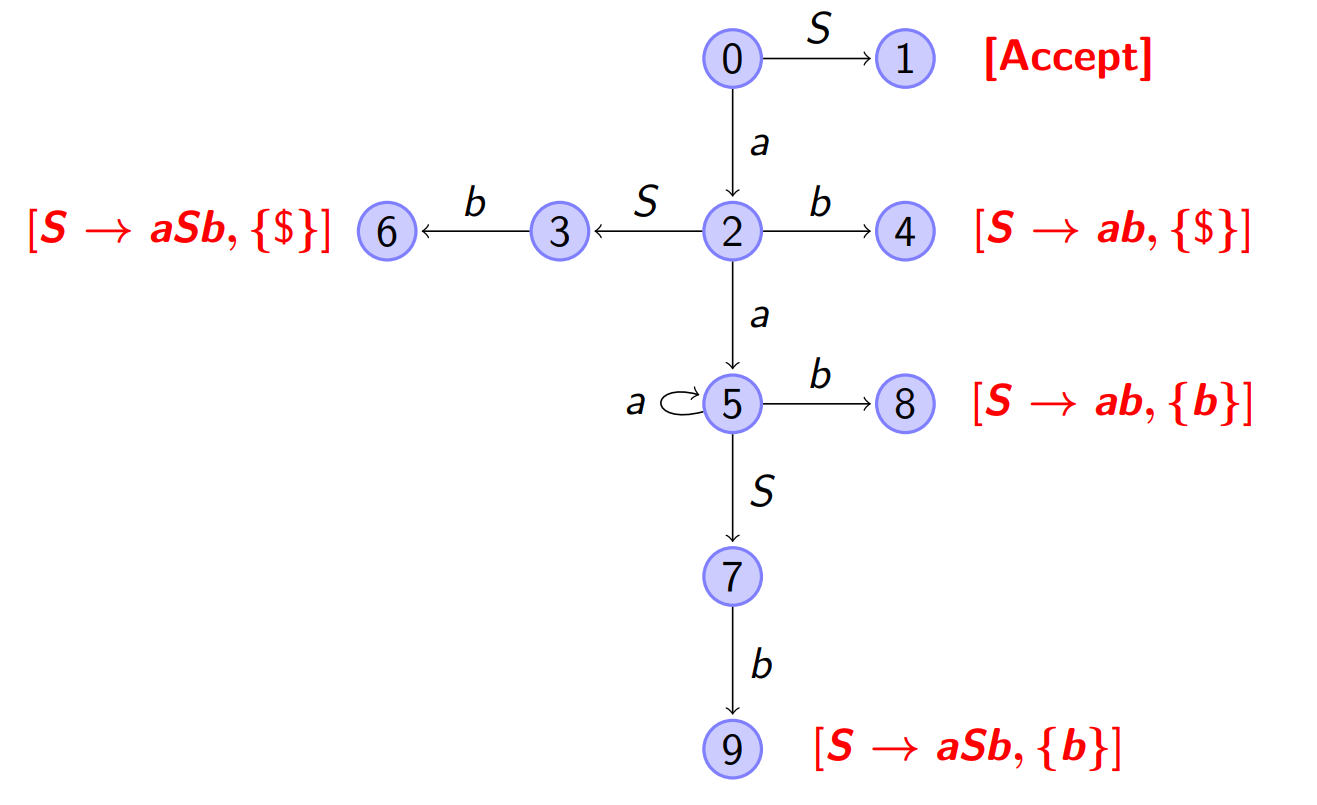
\includegraphics[width=\textwidth,keepaspectratio]{balanced-char_aut-lr1.png}
    \caption{Automa caratteristico LR(1) per Eq. \ref{balanced}}
    \label{balanced-char_aut-lr1}
\end{figure}
Lo utilizzeremo come guida per determinare, di volta in volta, quali mosse di shift e reduce applicare per verificare se una certa parola appartiene o no al linguaggio generato da \(\G\). 

\subsection{Procedura}
Consideriamo ad esempio la parola \(w = aaabbb\). Come prima cosa le applichiamo il carattere terminatore di stringa \(aaabbb\$\), e successivamente dobbiamo parlare delle strutture che utilizzeremo nella procedura, che saranno due pile:
\begin{itemize}
    \item nella prima inseriamo gli stati verso cui ci muoviamo;
    \item nella seconda conserviamo la derivazione parziale a cui siamo arrivati sinora.
\end{itemize}
Si tenga presente che in realtà potremmo farci bastare anche una sola pila, ma andrebbe a complicare sensibilmente la gestione della procedura.
\begin{itemize}
    \item Partiamo dallo stato \(0\) e inseriamolo nella pila degli stati;
    \item il primo simbolo che leggo in \(w\) è \(a\), vedo che l'automa presenta una \(a\)-transizione verso lo stato \(2\), per cui la eseguo, inserisco lo stato \(2\) nella pila, cancello il simbolo \(a\) appena "consumato" e passo al prossimo simbolo;
    \item il prossimo simbolo è ancora \(a\); di nuovo, eseguo la \(a\)-transizione verso lo stato \(5\), lo inserisco nella pila degli stati, elimino il simbolo consumato e vado avanti;
    \item abbiamo una terza occorrenza di \(a\) e abbiamo una \(a\)-transizione in forma di self loop in \(5\), che andiamo ad eseguire, reinserendo \(5\) nella pila degli stati e cancellando la nostra terza \(a\);
    \item troviamo quindi una \(b\), per cui ci spostiamo allo stato \(8\), il quale ha un'etichetta rossa, che riporta la formula \(S \to ab, \{b\}\); questo sta a indicare che, se abbiamo appena letto due simoli \(ab\), possiamo ritornare indietro di due passi, eliminando i due precedenti stati dalla pila e spostarmi direttamento dal primo \(5\) a \(7\), dal momento che i due stati sono collegati da una \(S\)-transizione:
    \begin{align*}
        \textrm{pila degli stati prima:} &\quad 02558 \\
        \textrm{pila degli stati dopo:} &\quad 0257 
    \end{align*}
    inoltre dobbiamo anche rimuovere gli ultimi due simboli \(ab\) dalla pila della derivazione e sostituirli con \(S\):
    \begin{align*}
        \textrm{pila di derivazione prima:} &\quad \#aaab \\
        \textrm{pila di derivazione dopo:} &\quad \#aaS 
    \end{align*}
    \item leggiamo un'altra \(b\) e avanziamo allo stato \(9\), e anche qui operiamo un passo di riduzione (reduce), nello specifico abbiamo che \(R: S \to aSb, \{b\}\); questo ci dice che dobbiamo tornare indietro di tre passi, eliminando i tre elementi precedenti sia nella pila degli stati e muovendoci verso \(3\), sia nella pila delle derivazioni; si osservi attentamente il cambiamento delle pile per capire cosa succede:
    \begin{align*}
        \textrm{pila degli stati prima:} &\quad 02579 & \textrm{pila di derivazione prima:} &\quad \#aaSb \\
        \textrm{pila degli stati dopo:} &\quad 023 & \textrm{pila di derivazione dopo:} &\quad \#aS
    \end{align*}
    \item proseguo quindi con la lettura e incontro una terza \(b\), mi muovo verso \(6\) e incontro una terza riduzione \(R: S \to aSb, \{\$\}\); di nuovo, torno indietro di tre stati e contestualmente sostituisco gli elementi nelle pile: 
    \begin{align*}
        \textrm{pila degli stati prima:} &\quad 0236 & \textrm{pila di derivazione prima:} &\quad \#aSb \\
        \textrm{pila degli stati dopo:} &\quad 0 & \textrm{pila di derivazione dopo:} &\quad \#S
    \end{align*}
    \item abbiamo terminato: ci troviamo nello stato \(0\) e troviamo solamente il nostro start symbol \(S\), che ci permette  muoverci verso lo stato \(1\), e l'endmaker \$; la presenza della keyword \(ACCEPT\) nello stato in cui abbiamo terminato ci indica che la parola è stata riconosciut dall'automa.
\end{itemize}

\subsection{Riassumendo}
Questo è un esempio del procedimento dell'algoritmo di shift/reduce; vediamo quali regole generali possiamo dedurne:
\begin{itemize}
    \item partendo dallo stato iniziale, inizio a leggere la parola data attraversando gli archi marchiati dalle \(symbol\)-transizioni che incontriamo di volta in volta;
    \item quando arrivo in un nodo in cui si dovrà effettuare un passo di riduzione, questo sarà marcato da un'etichetta che avrà la forma \(A \to B, \{l\}\); quello che dovrò fare a questo punto sarà scorrere all'indietro la pila delle derivazioni parziali e, se riesco a trovare un'occorrenza di quello stesso \(l\), (da capire e chiarire bene)
\end{itemize}
Gli automi caratteristici sono una rappresentazione utile, ma si tenga presente che la stessa funzione può essere ottemperata anche da una tabella.

\section{Costruzione dell'automa}
Dopo aver visto questo esempio, non possiamo fare a meno di domandarci com'è possibile per noi calcolare questo automa caratteristico e la relativa tabella di parsing.

\subsection{Stati}
Andiamo per prima cosa a vedere gli stati. Gli stati sono degli insiemi di items, dove gli items sono oggetti di diverso tipo e così definiti:
\begin{labeling}{LR(1)-items}
    \item[LR(0)-items] \(A \to \alpha \cdot \beta\)
    \item[LR(1)-items] [\(A \to \alpha \cdot \beta, L\)], dove \(L \subseteq T \cup \{\$\}\)\footnote{Ricordiamo che \(T\) è l'insieme dei terminali della grammatica considerata.}
\end{labeling}
Da qui capiamo finalmente cosa intendevamo quando prima abbiamo detto che gli LR(1)-items sono più ricchi dei loro equivaleenti LR(0), e ci permettono quindi di riconoscere più grammatiche. Coerentemente alla definzione sopra riportata, avremo che gli automi caratteristici LR(0) sono quelli i cui stati sono LR(0)-items, e analogamente per gli automi carattersitici LR(1).

Andiamo a fare subito un esempio per aiutarci a capire di cosa stiamo parlando. Consideriamo un LR(0)-item \(S' \to \cdot S\): il significato intuitivo è che, se siamo all'inizio della procedura di parsing, siamo in una posizione in cui vogliamo conoscere quali sono le parole derivabili a partire da \(S\), per cui è logico pensare che il nostro item \(S' \to \cdot S\) debba stare nello stato iniziale dell'automa, che chiamiamo \(P_0\).

Ma non sarà l'unico item a risiedere in \(P_0\). Per aiutarci, riprendiamo la nostra fidata grammatica in Eq. \ref{balanced}: in questo caso, analizzare la parola vuol dire aspettarsi qualcosa che derivi da \(aSb\) oppure \(ab\), per cui gli LR(0)-items di \(S\) saranno:
\begin{itemize}
    \item \(S \to \cdot aSb\);
    \item \(S \to \cdot ab\).
\end{itemize}
E verranno inseriti in \(P_0\).

\subsection{Chiusura di un insieme di LR(0)-items}
Andiamo ora a vedere il concetto di chiusura di un insieme di LR(0)-items:

\begin{definition}
    Sia \(P\) un insieme di LR(0)-items; allora, \(closure_0(P)\) è il più piccolo insieme che soddisfa la seguente equazione:
    \begin{equation}
        closure_0(P) = P \cup \{B \to \cdot \gamma \; \textrm{tale che} \; A \to \alpha \cdot B \beta \in closure_0(P) \; \textrm{e} \; B \to \gamma \in P'\}
    \end{equation}
\end{definition}

La chiusura consiste sostanzialmente in tutti quegli items che hanno un punto davanti ad un non terminale; poi, ricorsivamente, si vanno ad aggiungere tutte le chiusure dei terminali con un punto davanti.

\subsection{Esempio di calcolo della chiusura}
Prendiamo ora ad esempio la seguente grammatica:
\begin{align*}
    E \to& E+T \mid T\\
    T \to& T*F \mid F\\
    F \to& (E) \mid id
\end{align*}
e calcoliamo \(closure_0 (\{E' \to \cdot E\})\). Ecco il procedimento passo per passo:
\begin{enumerate}
    \item inizializziamo \(closure_0 (\{E' \to \cdot E\})\) = \(\{E' \to \cdot E\}\); 
    \item andiamo a vedere se questo insieme contiene qualche marker davanti ad un non-terminale: effettivamente c'è un marker prima di \(E\);
    \item aggiungiamo quindi le due produzioni di \(E\) alla chiusura \(\{E \to \cdot E+T\}\) e \(\{E \to \cdot T\}\);
    \item una volta aggiunte queste produzioni, vediamo ricorsivamente se si presentano altre situazioni con \(\cdot\);
    \item nel primo caso troviamo ancora \(\cdot E\) che però abbiamo già analizzato;
    \item nel secondo caso invece abbiamo \(\cdot T\) e non abbiamo ancora analizzato tutte le produzioni di \(T\), quindi andiamo ad aggiungere all'insieme le produzioni di \(T\);
    \item aggiungamo \(\{T \to \cdot T * F\}\) e \(\{T \to \cdot F\}\);
    \item ci troviamo di nuovo in un caso in cui abbiamo due nuove derivazioni con \(\cdot\) davanti
    ad un non-terminale, ma \(\cdot T\) è già analizzato, analizziamo quindi solo \(\cdot F\);
    \item aggiungiamo le produzioni di \(F\): \(\{F \to \cdot (E)\}\) e \(\{F \to \cdot id \}\).
    \item siamo arrivati alla conclusione, sotto è riportato l'insieme chiusura che abbiamo trovato:
\end{enumerate}
\begin{align*}
    E'&\to \cdot E \\
    E  &\to \cdot E+T \\
    E  &\to \cdot T \\
    T  &\to \cdot T * F \\
    T  &\to \cdot F \\
    F  &\to \cdot (E) \\
    F  &\to \cdot id
\end{align*}

Ora che abbiamo visto un applicazione otteniamo lo pseudocodice dell'algoritmo per la
computazione della chiusura:
\begin{figure}[H]
    \centering
    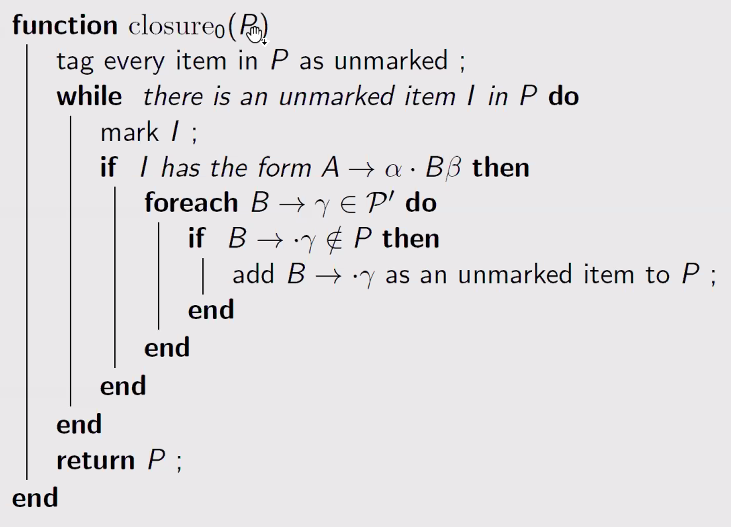
\includegraphics[width=.8\textwidth]{bottom-up-parsing_closure_algorithm.png}
    \caption{Algoritmo per il calcolo di \(closure_0(P)\)}
\end{figure}
\subimport{assets/pseudocode/}{lr0-closure.tex}

\subsection{Costruire un automa caratteristico per il parsing LR(0)}

Vedremo ora come costruire un automa caratteristico per il parsing di tipo LR(0) data una certa grammatica.

La tecninca di costruzione è incrementale: andiamo a popolare un set di stati definendo mano a mano la funzione di transizione, fino alla saturazione; il lettorè si accorgerà che tale tecnica è poi utilizzata per costruire anche altri automi LR.

In primis definiamo lo stato iniziale come \(P_0 = closure_0 (\{S' \to \cdot S\})\), dove \(S'\) è un carattere inserito da noi, mentre \(S\) è lo starting symbol della nostra grammatica.

Esisterà tra gli stati che abbiamo già collezionato uno stato \(P\) che contiene un item \(A \to \alpha \cdot x \beta\), che rappresenta uno stato in cui ho già visto \(\alpha\) e posso fare una transizione a \(x\beta\).

Esiste quindi una transizione da \(P\) ad uno stato \(P'\) che contiene l'item \(A \to \alpha x \cdot \beta\); se \(x\) è un terminale tale transizione rappresenta un'operazione di shift (come abbiamo visto nell'esercizio della sezione scorsa). 
Questo significa che avrò una transizione etichettata con \(x\) che mi porta da \(P\) a \(P'\).

Una volta che genero uno stato \(P'\) che contiene l'item \(A \to \alpha x \cdot \beta\) devo anche includervi tutti gli item che appartengono a \(closure_0 (\{ A \to \alpha x \cdot \beta \})\), poiché se \(\beta\) è un non terminale allora mi aspetto di poter trovare in \(P'\)  anche tutto ciò che deriva da \(\beta\).

Osserviamo subito un esempio di costruzione  di un automa caratteristico per il parsing LR(0).

\subsubsection{Esempio costruzione automa caratteristico LR(0)}
\label{esercizio_costruzione_automa_lr0}
Costruiamo l'automa caratteristico per il parsing LR(0) della seguente grammatica:
\begin{align*}
    S &\to aABe \\
    A &\to Abc \mid b \\
    B &\to d
\end{align*}
Partiamo con il creare lo stato iniziale, lo stato 0:
\begin{equation*}
    S' \to \cdot S
\end{equation*}
Ma non è concluso qui, infatti nello stato iniziale va anche la \(closure_0(\{ S' \to \cdot S \})\), quindi aggiungo le produzioni di \(S\): \(S \to \cdot aABe\).
Dato che non sono presenti altre produzioni con marker prima di caratteri non-terminali lo stato 0 è completo.

A questo punto ci troviamo nello stato 0 ed abbiamo due produzioni, una con il marker prima di \(S\) ed una con il marker prima di \(a\), dobbiamo aggiungere i seguenti due stati:
\begin{enumerate}
    \item \(\tau (0, S) =\) 1
    \item \(\tau (0, a) =\) 2
\end{enumerate}
Nota: gli stati possono venire indicati con la notazione 
\begin{equation*}
    \tau( \textrm{stato di provenienza}, \textrm{transizione di provenienza}).
\end{equation*}
Questi stati però potrebbero essere già presenti! Non è questo il caso dato che sono i primi stati che troviamo, ma in seguito dovremmo ricordarci di tale controllo.
\\
Partiamo con l'analizzare il nuovo stato \(\tau (0, S) =\) 1. \\
Dobbiamo calcolare il \emph{kernel} dello stato, che si ottiene spostando il marker oltre al carattere che ci ha portati qui:
\begin{equation*}
    S' \to S \cdot
\end{equation*}
Questo è quello che viene definito kernel dello stato; non presenta ulteriori transizioni possibili dato che il marker è arrivato in fondo, quindi passiamo ad analizzare un altro stato.
\\
Andiamo ad analizzare lo \(\tau (0, a) =\) 2. \\
Il kernel questa volta è
\begin{equation*}
    S \to a \cdot ABe
\end{equation*}
Dato che il kernel presenta almeno una produzione con un non-terminale alla destra del marker, dobbiamo aggiungere la chiusura del kernel a questo stato, ovvero:
\begin{align*}
    A &\to \cdot Abc\\
	A &\to \cdot b
\end{align*}
Quindi gli item dello stato 2 sono:
\begin{align*}
    S &\to a \cdot ABe\\
    A &\to \cdot Abc\\
	A &\to \cdot b
\end{align*}
Dallo stato 2 avremo quindi due possibili transizioni, una tramite \(A\) ed una tramite \(b\).
\\
Partiamo ad analizzare \(\tau (2, A) =\) 3. \\
Il kernel di questo stato è composto da due produzioni, dato che da 2 si può arrivare in 3 tramite due distinte produzioni:
\begin{align*}
    S &\to aA \cdot Be \\
    A &\to A \cdot bc
\end{align*}
Per verificare se questo stato è già astato raggiunto vado a verificare che non siano presenti stati con gli stessi item; non ve ne sono, lo stato 3 non è ancora stato effettivamente aggiunto quindi lo tengo.

Calcoliamo la chiusura dello stato, che ci porta ad aggiungere la seguente produzione:
\begin{equation*}
    B \to \cdot d
\end{equation*}
Una volta calcolata la chiusura, mi segno i nuovi stati da visitare.
\begin{itemize}
    \item \(\tau (3, B) =\) 5
    \item \(\tau (3, b) =\) 6
    \item \(\tau (3, d) =\) 7
\end{itemize}
\noindent Analizziamo ora lo stato \(\tau (2, b) =\) 4. \\
Questo stato ha come kernel
\begin{equation*}
    A \to b \cdot
\end{equation*}
che non presenta ulteriori possibili sviluppi, quindi passiamo oltre.
\\
Analizziamo lo stato \(\tau (3, B) =\) 5. \\
Il kernel in questo caso è
\begin{equation*}
    S \to aAB \cdot e
\end{equation*}
Tale kernel è già chiuso (la sua chiusura è vuota) e ci offre come unica transizione possibile \(\tau (5, e) =\) 8.
\\
Analizziamo lo stato 6 \( = \tau (3, B)\). \\
Il kernel è
\begin{equation*}
    A \to Ab \cdot c
\end{equation*}
Anche questo kernel è già chiuso; ci offre la transizion allo stato 9 \(= \tau (6, c)\).
\\
Analizziamo lo stato \(\tau (3, d) =\) 7. \\
Ha come kernel
\begin{equation*}
    B \to d \cdot 
\end{equation*}
Tale kernel è chiuso e non presnta transizioni uscenti.
\\
Non ci rimane che analizzare gli stati 8 e 9 che presentano rispettivamente i seguenti kernel:
\begin{align*}
    S &\to aABe \cdot \\
    A &\to Abc \cdot
\end{align*}
i quali non presentano ulteriori transizioni.

In conclusione l'automa caratteristico che otteniamo da questo procedimento può essere visualizzato in Fig.\ref{charateristic-automata_cosntruction}
\begin{figure}
    \centering
    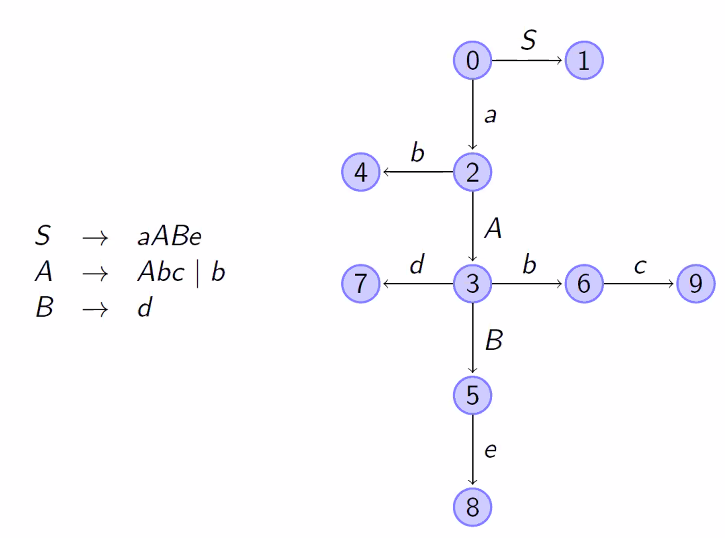
\includegraphics[width=.8\textwidth]{charateristic-automata_cosntruction.png}
    \caption{Automa caratteristico LR(0) per la grammatica \ref{esercizio_costruzione_automa_lr0}}
    \label{charateristic-automata_cosntruction}    
\end{figure}

Una volta terminata questa arzigogolata esercitazione possiamo dare un'occhiata all'algoritmo per la costruzione di un automa LR(0) in Alg.\ref{alg:char-automata}.
\begin{figure}
    \centering
    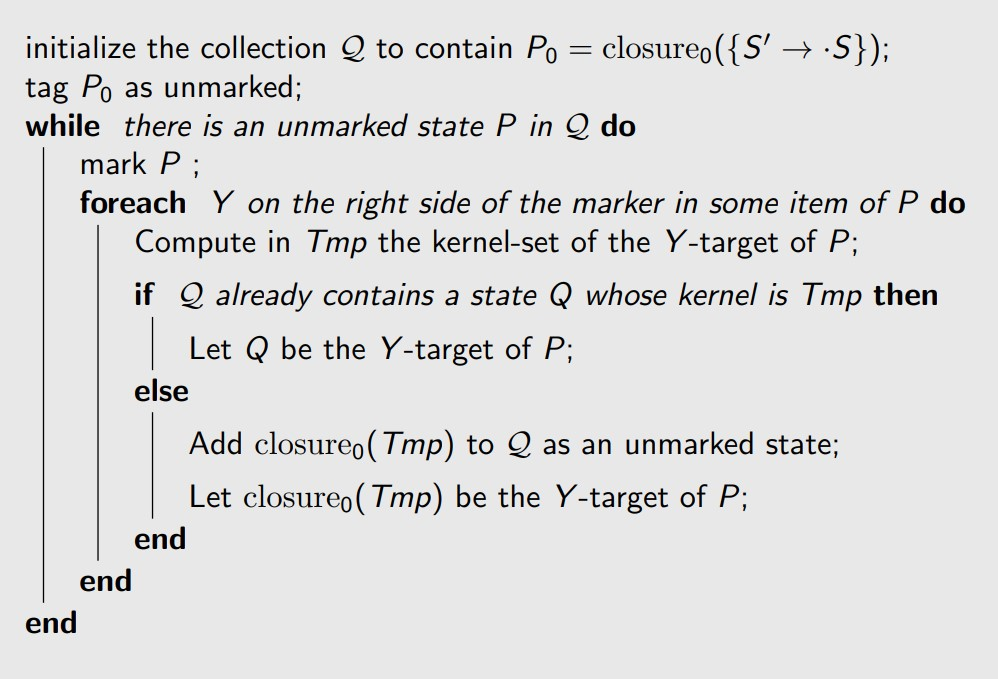
\includegraphics[width=.8\textwidth]{lr0-automata_construction_algorithm.jpg}
    \caption{Algoritmo per la costruzione di un automa LR(0)}
    \label{lr0-automata_construction_algorithm}    
\end{figure}
\subimport{assets/pseudocode/}{char-automata.tex}

Ma dove sono finite le etichette rosse che sull'automa dell'esercizio di shift/reduce ci segnalavano le mosse di reduce?
Lo scopriremo nella prossima sezione.


\section{Parsing table per bottom-up}

L'algoritmo di shift/reduce compie delle mosse in base a cosa leggiamo sulle due pile (pila del parsing e pila della lettura). L'algoritmo usa una tabella di parsing per muoversi.

La tabella ha tante righe quanti gli stati dell'automa caratteristico, ed una colonna per ogni simbolo in \(V \cup \{ \$ \}\).
Nota che la tabella dipende dall'automa caratteristico, automi diversi portano a tabelle diverse che portano a tipi di parsing diversi.

Le mosse di shift dipendono direttamente dalla funzione di transizione dell'automa; mentre le mosse di reduce sono più articolate: vanno effettuate solo quando raggiungiamo quei particolari stati etichettati ed implicano poi il dover cancellare degli elementi dalla pila degli stati e dalla pila di lettura per poi inserire altri caratteri in quest'ultima pila.

Le mosse di reduce dipendono dal contenuto degli stati dell'automa: in un certo stato della tabella di parsing andiamo ad inserire una mossa di riduzione se la produzione \(A \to \beta\) è effettuata in uno stato contenente un reducing item per \(A \to \beta\), ma cosa sono i reducing item?
\begin{itemize}
    \item Item \(A \to \beta \cdot \) nel caso di item LR0 (ovvero quando sono arrivato alla fine della produzione di \(\beta\));
    \item item \(A \to \beta \cdot, \; \Delta\) nel caso LR1 (ovvero quando ho terminato l'analisi del body di \(\beta\)).
\end{itemize}
Le riduzioni dipendono dalla lookahead function \(\mathcal{LA}\) che è definita per tutte le coppie \((P,\; A \to \beta)\) tali che \(P\) contiene un reducing item per \(A \to \beta\).

Da mensionare il fatto che la scelta dell'automa e della lookahead function per la costruzione della parsing table sono le caratteristiche che distinguono le varie tecniche di bottomup parsing.
Nello specifico abbiamo le seguenti conseguenze:
\begin{itemize}
    \item la classe delle grmmatiche analizzabili dipene dalla scelta appena menzionata;
    \item anche la dimensione della parsing table dipende da tale scelta;
    \item la procedura di riempimento della parsiing table è invece indipendente;
    \item anche l'algoritmo di parsing è sempre uguale.
\end{itemize}

\subsection{Costruire una parsing table per il bottom-up parsing}

Vediamo ora nello specifico come costruire una parsing table.
Dobbiamo riempire ogni entry \((P, Y)\) seconndo le seguenti regole:
\begin{itemize}
    \item se \(Y\) è un terminale e \(\tau (P,Y)=Q\) inserisci la mossa "shift Q";
    \item se \(P\) contiene un reducing itemp per \(A \to \beta\) e \(Y \in \mathcal{LA}(P, A \to \beta)\), inserisci la mossa "reduce \(A \to \beta\)";
    \item se \(P\) contiene l'accepting item e \(Y=\$\) inserisci "accept";
        \begin{itemize}
            \item nel caso degli automati LR(0) l'item è \(\{S' \to S \cdot\}\);
            \item nel caso degli automati LR(1) l'item è \(\{S' \to S \cdot, \; \Delta\}\);
        \end{itemize}
    \item se \(Y\) è un terminale o \$ e nessuna delle condizioni precedenti è valida, inserisce "errore";
    \item se \(Y\) è un non-terminale e \(\tau (P, Y)=Q\) inserisci la mossa "goto \(Q\)".
\end{itemize}


\end{document}